\mbox{}


\chapter{Entrenamiento del modelo mediante Google Colab}
\label{ch:chapter2}
Uno de los parámetros más importantes dentro dentro del entrenamiento de modelos de deep learning es la velocidad.
La velocidad de entrenamiento es de vital importancia ya que los modelos pueden requerir entradas de tamaño masivo, por lo que la capacidad de cómputo
va a ser clave para acelerar este proceso y poder enfocarnos plenamente a la mejora del rendimiento de nuestro modelo, sin tener como cuello de botella la espera
que nos pueda producir volver a entrenar el mismo con distintos parámetros.
De este modo podemos reajustar constantemente nuestro modelo para encontrar el punto óptimo de manera ágil.
En este trabajo vamos a entrenar nuestro modelo haciendo uso del framework de código abierto de Tensorflow, el cual incluye una API de deep learning llamada Keras, que será la que utilicemos.

El tipo de operaciones que requiere nuestra aplicación en la parte del tratamiento de imágenes y los propios procedimientos que realizan las redes neuronales
para hacer sus cálculos son operaciones matriciales.
Nuestro objetivo será aprovechar al máximo el rendimiento que una GPU nos puede dar en este tipo de operaciones gracias
a su arquitectura de paralelización, ya que es la idónea para este tipo de trabajo.
La ventaja que nos da frente a la cpu es la capacidad de cómputo, gracias a su conectividad por PCI express y el ancho de banda que esta proporciona.

\begin{figure}
    \centering
    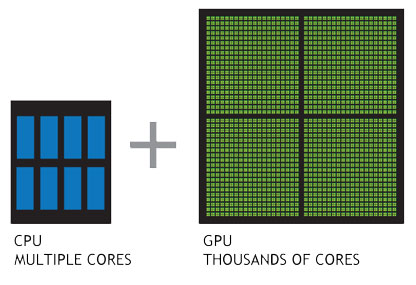
\includegraphics[width=0.5\textwidth]{images/chapter2/cpu-and-gpu.jpg}
    \caption{Arquitectura de paralelización de una GPU.}
    \label{fig:Arquitectura de paralelización de una GPU}
\end{figure}


\section{Modelo propuesto}\label{sec:modelo-propuesto}
En esta parte del trabajo se pretende conseguir la máxima velocidad de entrenamiento posible manteniendo unos niveles de precisión elevados en la predicción.
Nuestro modelo tiene como cometido primordial poder clasificar distintas imágenes según el estado del terreno que aparece en la fotografía, siendo las opciones : terreno dañado y
terreno en buenas condiciones.
Para ello disponemos de un dataset de 268 imágenes multiespectrales ( describir dataset, procedencia ee imagen multiespectral).
Como framework principal para realizar el entrenamiento nos ayudaremos de Tensorflow que incluye la librería de deep learning Keras, la cual simplifica mucho la implementación de este tipo de algoritmos de
aprendizaje automático gracias a que sus objetos y funciones están construidos de una manera intuitiva.
La distribución a efectuar sobre el conjunto de datos en entrenamiento y test es del 70 y 30 por ciento respectivamente.
Para la construcción de este algoritmo haremos uso de las siguientes capas, sobre las que Tensorflow nos da una API para tener control total sobre su configuración.

\begin{itemize}
    \item \textbf{Conv2D}: Capa convolucional cuyo principal objetivo es extraer características de la imagen de entrada o partes de la misma.
    El térmido 2D se refiere al movimiento del filtro, el cuál es un parámetro de entrada de este tipo de capas.
    El filtro atraviesa la imagen en dos dimensiones.
    Tiene como requisitos una imagen en tres dimensiones, el número de filtros que vamos a aplicar sobre la imagen.
    Aplicaremos sobre esta capa una configuración de 64 filtros y un tamaño de Kernel de 3x3 ya que nuestras imágenes son de 128x128 píxeles para ayudar a nuestro modelo a mejorar su aprendizaje con filtros de mayor tamaño.
    \item \textbf{Activación Relu ( Recitified Linear Unit )}: En redes neuronales, una función de activación es la responsable de transformar la entrada. Sus principales funciones son detectar posibles correlaciones entre dos variables distintas dependiendo de sus valores y ayudar al modelo a tener en cuanta efectos no lineales, lo que significa ( clarificar efectos no lineales.)
    Como podemos observar en la figura~\ref{fig:Función de activación Relu} la función de activación Relu se comporta devolviendo un 0 para valores de entrada negativos y en caso contrario devolviendo el propio valor de entrada. (razones por las que funciona bien)
    \item \textbf{MaxPooling2D}: Se presenta la arquitectura de Google Cloud diseñada para soportar toda la infraestructura de la aplicación y se explica la puesta en producción del servicio.
    \item \textbf{Dropout}: Se preparan los distintos frameworks web que van a ser puestos a prueba haciendo uso del lenguaje de programación Python.
    \item \textbf{Flatten}: Se presentan los resultados obtenidos mediante las pruebas de carga y también algunas posibles líneas de trabajo futuro que se pueden desempeñar en relación al presente trabajo.
    \item \textbf{Dense}:
    \item \textbf{Optimizador Adam}:
    \item \textbf{Hiperparámetros}:
\end{itemize}


\begin{figure}
    \centering
    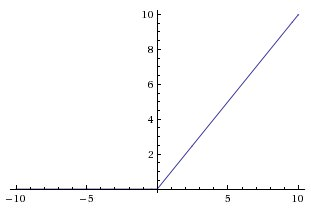
\includegraphics[width=0.5\textwidth]{images/chapter2/relu.jpg}
    \caption{Función de activación Relu.}
    \label{fig:Función de activación Relu}
\end{figure}
Además, realizaremos algunas optimizaciones a nivel de hardware para acelerar el proceso de forma general.

\begin{itemize}
    \item \textbf{Uso de variables de 16 bits en vez de 32 bits}: Una de las posibilidades que nos brinda el uso de una GPU es reducir a la mitad el uso en memoria de las variables del proceso.
    Usaremos esto siempre y cuando no afecte al rendimiento en cuanto a predicción.
    \item \textbf{Uso del compilador XLA}: El compilador XLA (Accelerated Linear Algebra) optimiza el grafo de nuestro modelo de manera específica haciendo uso de la GPU.
    \item \textbf{Valores altos del parámetro de entrenamiento BatchSize}: Gracias a la capacidad de cómputo de nuestra tarjeta gráfica podemos permitirnos el uso de valores altos en este parámetro de entrenamiento.
\end{itemize}


\section{Entorno Google Colab}\label{sec:entorno-google-colab}
La plataforma de Google Colab es un servicio gratuito de google, mediante el cual podemos ejecutar e instalar librerías del lenguaje de programación python.
Una de las grandes ventajas de trabajar con este tipo entorno es que no necesitamos configuración ninguna, se ejecuta de forma íntegra en el navegador sin necesidad de instalar nada previamente y podemos compartir
nuestro trabajo con otras personas.
Estas características permiten a Google Colab convertirse en una utensilio muy válido para personas que están dando sus primeros pasos en este área de la inteligencia artificial, pero haciendo uso
de unas herramientas profesionales.
En este trabajo haremos uso de la tarjeta gráfica Tesla K80.
Las características primarias de nuestro principal unidad de cómputo son las siguientes :
\begin{itemize}
    \item 4992 núcleos de NVIDIA CUDA con diseño de dos GPU
    \item Hasta 2,91 teraflops de rendimiento en operaciones de precisión doble con NVIDIA GPU Boost.
    \item 24 GB de memoria GDDR5
    \item 480 GB/s de ancho de banda de memoria agregado.
    \item Hasta 8,73 teraflops de rendimiento en operaciones de precisión simple con NVIDIA GPU Boost.
\end{itemize}
El uso de este tipo de herramientas en esta plataforma es extrapolable a otras nubes sin las restricciones en cuanto al número de unidades de procesamiento que necesitamos,
la interoperabilidad de sus elementos con otros componentes externos, tales como servidores o respositorios de código y la configuración explícita de cada uno de los entornos de ejecución.
Una de las mejores faces que tiene poder usar un entorno como Google Colab es que el servicio se ejecuta de manera íntegra online, de modo que toda la carga computacional reside en la herramienta de google y no en
nuestro computador, permitiendo así poder trabajar de manera fluida realizando otro tipo de cometidos en nuestra máquina o simplemente ejecutando un proceso para el cual no tenemos suficiente potencia disponible.
